
\documentclass[a4paper,12pt]{article}
\usepackage{geometry}
\geometry{a4paper, margin=1in}
\usepackage{longtable}
\usepackage{colortbl}
\usepackage{xcolor}
\usepackage{setspace}
\usepackage{graphicx}
\usepackage{amssymb}
\setstretch{1.2}
\usepackage{xepersian}
\settextfont{Vazirmatn}
\definecolor{headerblue}{RGB}{44, 62, 80}

\begin{document}

% هدر و لوگو
\begin{center}
    % اگر لوگو دارید، مسیر فایل را جایگزین کنید
    % 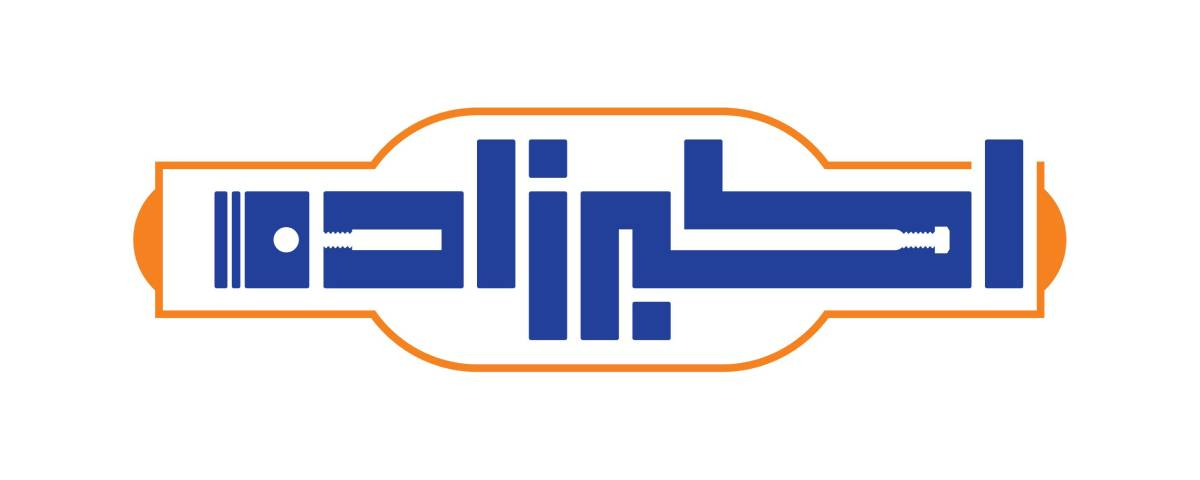
\includegraphics[width=3cm]{logo.png} \
    {\Huge \textbf{به‌نام اکبرزاده}} \
    {\large فاکتور فروش}
\end{center}

\vspace{0.5cm}

% اطلاعات مشتری و سفارش
\noindent
\begin{tabular}{|p{7cm}|p{7cm}|}
\hline
\textbf{شماره:} 14040404002 & \textbf{تاریخ:} 17:33 - 1404/04/04 \
\hline
\textbf{ساعت:} 17:33 & \textbf{مشتری:} مهیار اکبرزاده \\
\hline
\textbf{موبایل:} 09144588587 & \textbf{آدرس:} ایثار \\
\hline
\end{tabular}

\vspace{0.5cm}

% جدول کالاها
\begin{longtable}{|c|c|p{4cm}|c|c|c|c|}
\hline
\rowcolor{headerblue} \color{white}
\textbf{ردیف} & \textbf{کد کالا} & \textbf{شرح} & \textbf{مقدار} & \textbf{واحد} & \textbf{فی} & \textbf{قیمت کل} \
\hline
\endhead
1 & 0020200944 & نيم موتور 405 & 2 & عدد & 200 & 400 \\
\hline
\end{longtable}

% جمع کل و بخش پرداخت
\vspace{0.3cm}
\noindent
\begin{tabular}{|p{7cm}|p{7cm}|}
\hline
\textbf{جمع کل کالاها و خدمات:} & 400 ریال \\
\hline
\textbf{تخفیف:} & 0 ریال \\
\hline
\textbf{مالیات/عوارض:} & 0 ریال \\
\hline
\textbf{مبلغ قابل پرداخت:} & 400 ریال \\
\hline
\end{tabular}

\vspace{0.3cm}

% نحوه تسویه
\noindent
\textbf{نحوه تسویه:}
\begin{tabular}{|c|c|c|c|}
\hline
نقد & چک & تسویه & کارتخوان \\
\hline
 &  &  &  \\
\hline
\end{tabular}

\vspace{0.5cm}

% توضیحات و مهر و امضا
\noindent
\textbf{توضیحات:} ...............................................................................................

\vspace{1.5cm}

\noindent
مهر و امضا خریدار \hspace{8cm} مهر و امضا فروشنده

\vfill

% متن پایین صفحه
\noindent
کالاهای مندرج در این فاکتور تا تسویه حساب کامل نزد مشتری امانت می‌باشد.

\end{document}
